\chapter{Aufgabe 11 - Monitoring}
\section{Unterschiedliche Ansätze des Monitorings}
\begin{table}[ht]
    \centering
    \begin{tabular}{ p{3cm} | p{4cm} | p{5cm} }
         \textbf{Monitoring Ansatz}&
         \textbf{Vorteile} &
         \textbf{Nachteile} \\
         
         \hline
         \hline
         \multirow[c]{4}{=}{\textbf{Software-Monitoring}} &
         \begin{itemize}
             \item Einfach zu implementieren
             \item Keine zusätzliche Hardware erforderlich
         \end{itemize} &
         \begin{itemize}
             \item Zugriff auf Kernel-Ebene benötigt
             \item Höherer Zeitbedarf und Ressourcennutzung
             \item Möglicherweise veraltete Daten
             \item (mögliche) Beeinträchtigung des Echtzeit-Verhaltens
         \end{itemize} \\

         \hline
         \multirow[c]{4}{=}{\textbf{Hybrid-Monitoring}} &
         \begin{itemize}
             \item Geringerer CPU-Overhead
             \item Gute Balance zwischen Kosten/Genauigkeit
         \end{itemize} &
         \begin{itemize}
             \item Zusätzliche Hardware benötigt
             \item Anpassungen im Quellcode notwendig
         \end{itemize} \\

         \hline
         \multirow[c]{4}{=}{\textbf{Hardware-Monitoring}} &
         \begin{itemize}
             \item Unabhängig, da keine Systemressourcen benötigt werden
         \end{itemize} &
         \begin{itemize}
             \item Zusätzliche Hardware benötigt
             \item Spezielles Werkzeug notwendig aufgrund der Größe
         \end{itemize}
    \end{tabular}
\end{table}
\newpage
Das Software-Monitoring ist zwar einfach zu implementieren, jedoch verliert es in Sachen Performance und Genauigkeit, da die Daten über mehrere Ebenen durchgereicht werden und zudem eine Umwandlung von analog in digital geschieht, wodurch es zu Ungenauigkeiten kommt.

Beim Hybrid-Monitoring ist die Balance zwischen Leistung/Effizienz.
Die eigentliche Messung geschieht über Hardware-Sensorik, jedoch muss der Quellcode angepasst werden, um diese Daten auslesen zu können.
Daher bietet sich dies als Kompromiss an, falls Leistung \glqq über\grqq ist.

Das Hardware-Monitoring ist am schnellsten, da keine zusätzlichen Ebenen benötigt werden, um die Daten auszulesen.
Zudem ist die Genauigkeit ebenfalls höher, da die analogen Signale nicht in digitale umgewandelt werden müssen.

\section{Konzept eines Software-Monitoring für 8051}
\paragraph{eine Stunde}
Unsere Idee ist im internen RAM je Task vier Byte zu reservieren.
Timer 1 zählt dann zur Laufzeit des jeweiligen Tasks mit.
Wenn der Task gewechselt wird, wird die gelaufene Zeit aufaddiert und die Zellen gewechselt.
Damit können wir einen unsigned integer mit 32-Bit speichern, dessen Wert in ms ca. einer Stunde und zwölf Minuten entspricht.

\paragraph{sechs Monate}
Das Vorgehen entspricht dem vorherigen.
Dafür benötigen wir ca. 5,5 Byte.
Diese runden wir auf sechs Byte auf.
Mit dieser Anzahl wären wir sogar in der Lage 108 Monate zu speichern.

\section{Laufzeitsimulation}
\begin{figure}[ht]
    \centering
    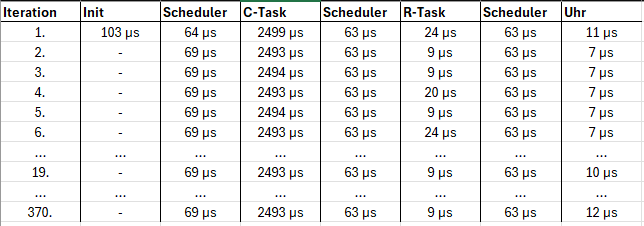
\includegraphics[width=\linewidth]{ressources/aufgabe11/Beispieliterationen mit Extrapolation.png}
    \caption{Laufzeiten der Tasks mit Extrapolation}
    \label{fig:iterationMitExtrapolation}
\end{figure}

\begin{figure}[ht]
    \centering
    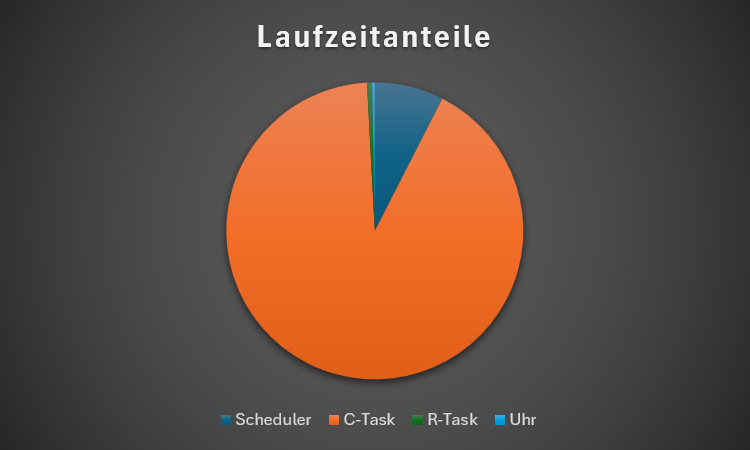
\includegraphics[width=0.9\linewidth]{ressources/aufgabe11/Laufzeitanteile.png} 
    \caption{Laufzeitanteile}
\end{figure}

\begin{figure}
    \centering
    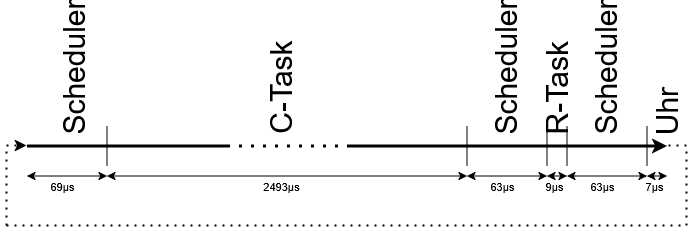
\includegraphics[width=\linewidth]{ressources/aufgabe11/Zeitverlauf_Beispiel.png}
    \caption{Zeitverlauf wiederkehrend}
\end{figure}